\textbf{N-Gram Graph} (NGG) is a NLP tool, initially proposed by George Giannakopoulos \cite{Ngram}, that uses word or character n-grams in order to achieve documents summarization. The NGG tool basically slices the text in words or characters n-grams and represent them in a graph \emph{G = $\lbrace N,E,L,W\rbrace$} according to the following structure:
\begin{itemize}
	\item N is the set of nodes created for every different n-gram in the text;
	\item E represent the edge of the graph; two nodes are connected if they are "close'' or within a \emph{distance window} from each other. The distance windows is denominated as \emph{neighbourhood distance};
	\item L is a labelling function which assigns labels to every node and every edge (define the size of the n-gram);
	\item W is the weight function which assigns weights to every edge according to the number of times that two n-gram appear close one to the other.
\end{itemize}

The big advantage due to use of this methodology is language
independence, since it makes no assumption on the underlying languages and
allows text manipulation through graph operations.

In particular three operations are mandatory for our goal:
\begin{itemize}
	\item the \textbf{Merging or Union } operator that, given two graphs $G_1$ and $G_2$, returns a graph with all the edges, both common and uncommon, of the two operand graphs. The edges weights are the average of the original ones;
	\item the \textbf{Intersection} operator between two graphs $G_1$ and $G_2$, which returns a graph with only the common edges of $G_1$ and $G_2$ with averaged weights;
	\item the \textbf{Normalized Value Similarity}[NVS] function that, for every n-gram rank, indicates how many of the edges contained in graph $G_i$ are also contained in graph $G_j$, considering also the weights of the matching edges and normalizing the result with respect to the graph size.
\end{itemize}

In particular $NVS(G_i,G_j) = \frac{VS(G_i,G_j)}{SS(G_i,G_j)}$ where:
\begin{equation}
 VS(G_i,G_j)=\frac{\sum e \in G_i \frac{\min(w_e^i, w_e^j)}{\max(w_e^i, w_e^j)}}{\max(\mid G_i \mid, \mid G_j \mid)}
\end{equation}

\begin{equation}
 SS(G_i,G_j)=\frac{\min(\mid G_i \mid, \mid G_j \mid)}{\max(\mid G_i \mid, \mid G_j \mid)}
\end{equation}

A fourth operation is used to filter out baseline events from the set of the news inside the contradiction window:
\begin{itemize}
 	\item the \textbf{Degrade} function, that reduces the weight of particular edges of graph $G_1$ with respect to the common edges of graph $G_2$. Common edges are the ones that identify a base knowledge that is independent from the contradiction window.
\end{itemize}

In this research work, NGG tool is used to compute both the tweet-news correlation and to create a summary of the most significant event that caused the contradiction. 
The work-flow of this computation is split in different phases.

\subsubsection*{Tweet-News Correlation}
To compute the correlation between contradiction tweets and news, this methodology exploits the base idea of using the NVS similarity as a correlation function: the higher is the similarity between tweets graph representation and news graph, the higher will be the correlation.

More in detail, this procedure performs the following step:
\begin{itemize}
	\item computes the graph representation of the contradiction tweets (cTweetGraph[i]);
	\item computes the  graph representation of all the news inside the contradiction windows (insideNews[i]).
\end{itemize}

Once we have these base components, we use an algorithm to create a background knowledge about each processed topic.

\begin{algorithmic}
\FOR{New nw : allNews}
	\IF{ nw outside contradiction window }
		\STATE nGraph = DocumentNGramGraph(nw.getText());
		\STATE double NVS = Similarity(nGraph, insideNews[i]);
		\IF{NVS < similarityLimit}
			\STATE outsideNews[i].merge(newsGraph);
		\ENDIF
	\ENDIF
\ENDFOR
\STATE baseline[i] = insideNews[i].degrade(outsideNews[i]);
\end{algorithmic}

Our approach is to filter out form the outsideNews those that belong to the group of the insideNews so as to avoid misleading results.
We have to take this precaution because with a fixed timeWindows some news related to the main event can fall in the outsideNews.
This produce bad result when we create the baseline graph as the degraded version of the insideNews respect the outsideNews, since the degrade function decrease the weight of the common edges between insideNews and outsideNews. In the previous pseudo code the similarityLimit is used to filter out the misleading news; this limit index has been detected empirically to 0.5, but this is reasonable since, in a single news the relevant information is for sure less than 100\% of the real content.

When we have a good baseline we can compute the correlation for the news inside the contradiction window.
\begin{algorithmic}
\FOR{News nw : allNews}
	\IF{nw inside contradiction window}
		\STATE nGraph = DocumentNGramGraph(nw.getText());
        \STATE nGraph = nGraph.intersectGraph(background[i]);
        \STATE correlationValue = Similarity(nGraph, cTweetGraph[i]);
	\ENDIF
\ENDFOR        
\end{algorithmic}

The NGG tool allows us to compute the similarity between text without the usage of grammar information and allow a controlled baseline removal function.
Of course such algorithm requires a lot of computation power, but it's justified by the added value of getting proper summary independent of the semantic of the new's text.

In figure \ref{fig:N-gram-expl} is possible to see how the algorithm work in a graphical way.

\begin{figure}[htbp]
	\centering
			{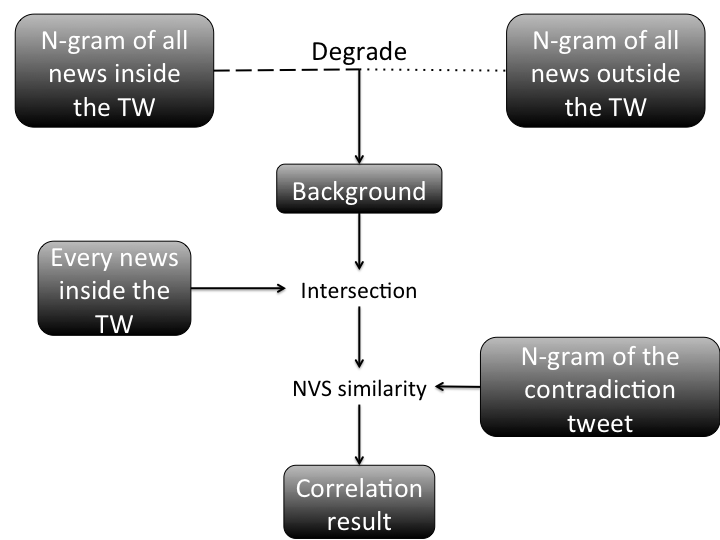
\includegraphics[width=8.5cm,height=7cm]{image/N-gram-expl.png}}	
		\caption[N-gram-expl]{Graphical explanation of how is computed the tweets-news correlation}
	\label{fig:N-gram-expl}
\end{figure} 

\subsubsection*{Summary Creation}
The second goal of this research is to create a summary of the event that cause the sentiment shift. 

For this purpose we use the news with the highest correlation value obtained at the step before.
Our choice was to limit the summary length to 150 word so there is no need to summarize many document. 

In particulate we select the candidate document to be summarized with the following procedure:
\begin{algorithmic}
\STATE stDev = standard deviation of the correlation values
\STATE sortNew[] = News sorted for decreasing correlation value
\FOR{i = 1 ; i < sortNew.length ; i++}
	\IF{ (i >=3) or (sortNew[i].getScore() <  (sortNew[0].getScore() - $stDev^2$))}
		\STATE sortNew.remove(i)
	\ENDIF
\ENDFOR
\end{algorithmic}

The aim of this procedure's step is to obtain at most three relevant news to summarize and the intersection of the selected news will never be empty since we intersect quite similar news.

The summary algorithm perform the following action:

\begin{algorithmic}
\STATE newSentence[] = sentence of the candidate document
\FOR{ String sentence : newSentence }
	\STATE sGraph = DocumentNGramGraph(sentence);
    \STATE score.setValue(Similarity(sGraph, cTweetGraph[i]));
    \STATE score.setSentence(sentence)
    \STATE scoredSentence.add(score)
\ENDFOR
\STATE Arrays.sort(scoredSentence);
\end{algorithmic}

create the summary using the sentence with the highest NVS value until we reach 150 word.

This algorithm create a summary composed by the most significant sentences in news with the highest correlation value using a back-loop approach, but is not able to remove redundant sentences. Even so, a summary composed by sentences results to be more human readable than a list of key word.



